              
% --------------------------------------------------------------
% This is all preamble stuff that you don't have to worry about.
% Head down to where it says "Start here"
% --------------------------------------------------------------
 
\documentclass[11pt]{article}
\usepackage[utf8]{inputenc} 
\usepackage[margin=1in]{geometry}
\usepackage{graphicx}
\usepackage{float}
\usepackage{hyperref} 
\usepackage{amsmath,amsthm,amssymb}
\usepackage[table]{xcolor}
\usepackage{biblatex}
\begin{filecontents*}{\jobname.bib}
@book{bestref,
  title={The dynamics of reinforcement learning in cooperative multiagent systems},
  author={Claus, Caroline and Boutilier, Craig},
  journal={AAAI/IAAI},
  number={s 746},
  pages={752},
  year={1998}
}
\end{filecontents*}
 
\addbibresource{\jobname.bib}
 
\newcommand{\N}{\mathbb{N}}
\newcommand{\Z}{\mathbb{Z}}
 
\newenvironment{theorem}[2][Theorem]{\begin{trivlist}
\item[\hskip \labelsep {\bfseries #1}\hskip \labelsep {\bfseries #2.}]}{\end{trivlist}}
\newenvironment{lemma}[2][Lemma]{\begin{trivlist}
\item[\hskip \labelsep {\bfseries #1}\hskip \labelsep {\bfseries #2.}]}{\end{trivlist}}
\newenvironment{exercise}[2][Exercise]{\begin{trivlist}
\item[\hskip \labelsep {\bfseries #1}\hskip \labelsep {\bfseries #2.}]}{\end{trivlist}}
\newenvironment{reflection}[2][Reflection]{\begin{trivlist}
\item[\hskip \labelsep {\bfseries #1}\hskip \labelsep {\bfseries #2.}]}{\end{trivlist}}
\newenvironment{proposition}[2][Proposition]{\begin{trivlist}
\item[\hskip \labelsep {\bfseries #1}\hskip \labelsep {\bfseries #2.}]}{\end{trivlist}}
\newenvironment{corollary}[2][Corollary]{\begin{trivlist}
\item[\hskip \labelsep {\bfseries #1}\hskip \labelsep {\bfseries #2.}]}{\end{trivlist}}
 
\begin{document}
 
% --------------------------------------------------------------
%                         Start here
% --------------------------------------------------------------
 
\setlength\parindent{0pt}
%\renewcommand{\qedsymbol}{\filledbox}
 
\title{Assignment 3: N-armed bandit problem}%replace X with the appropriate number
\author{Pierre Gérard (ULB)\\ %replace with your name
INFO-F-409 - Learning dynamics} %if necessary, replace with your course title
 
\maketitle

\section{N-Armed Bandit}
Like in the slides \textit{Multi-Agent Reinforcement Learning}, all graph have been averaged over 2000 iterations.


\subsection{Exercice 1}

\subsubsection{Average reward for each algorithm}

Two interpretations of this graph were possible:
\begin{itemize}
	\item the overall average reward for this algorithm, including the training. In other word for the play $t$, an average from $0$ to $t$,
	\item or the average reward for this algorithm at a precise moment. In other word, what is the reward at $t$.
\end{itemize}
The first one has been chosen because it take into account all "early failure".

\begin{figure}[H]
   \centering
   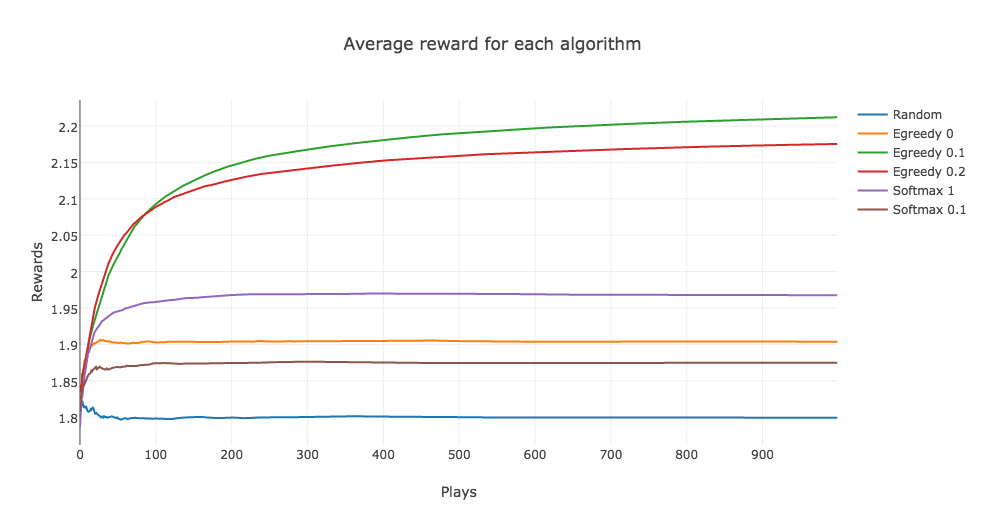
\includegraphics[width=0.8\textwidth]{img/1-1/reward.png}
\end{figure}

\subsubsection{Plot per arm}

\begin{figure}[H]
   \centering
   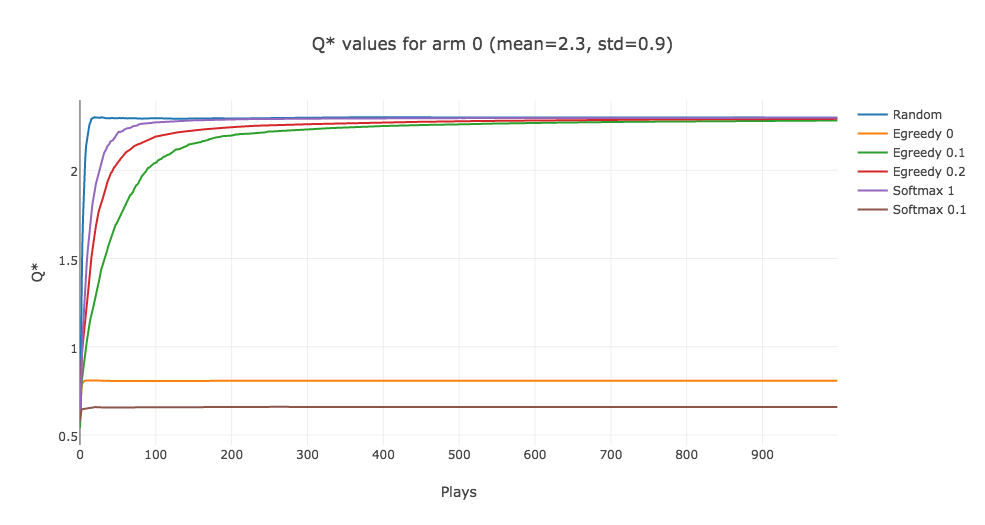
\includegraphics[width=0.7\textwidth]{img/1-1/q1.png}
\end{figure}

\begin{figure}[H]
   \centering
   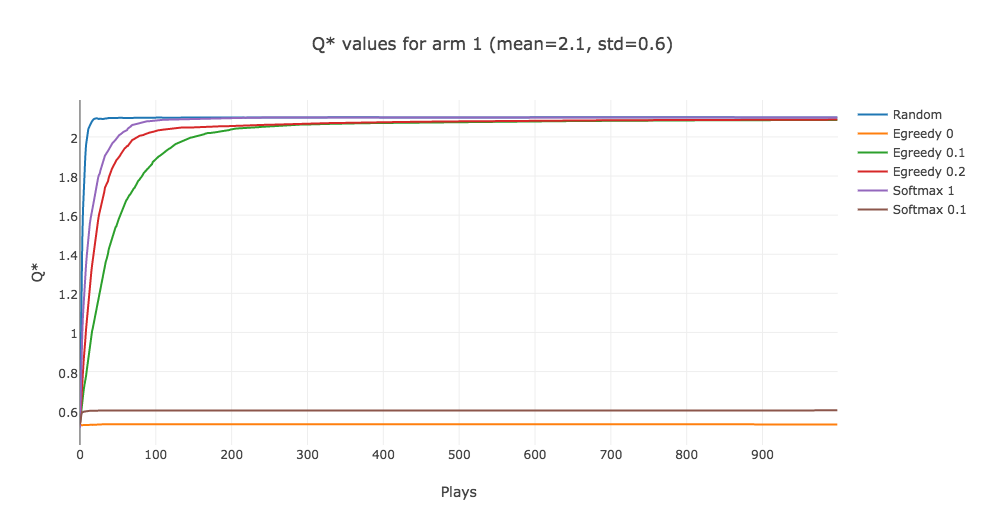
\includegraphics[width=0.7\textwidth]{img/1-1/q2.png}
\end{figure}

\begin{figure}[H]
   \centering
   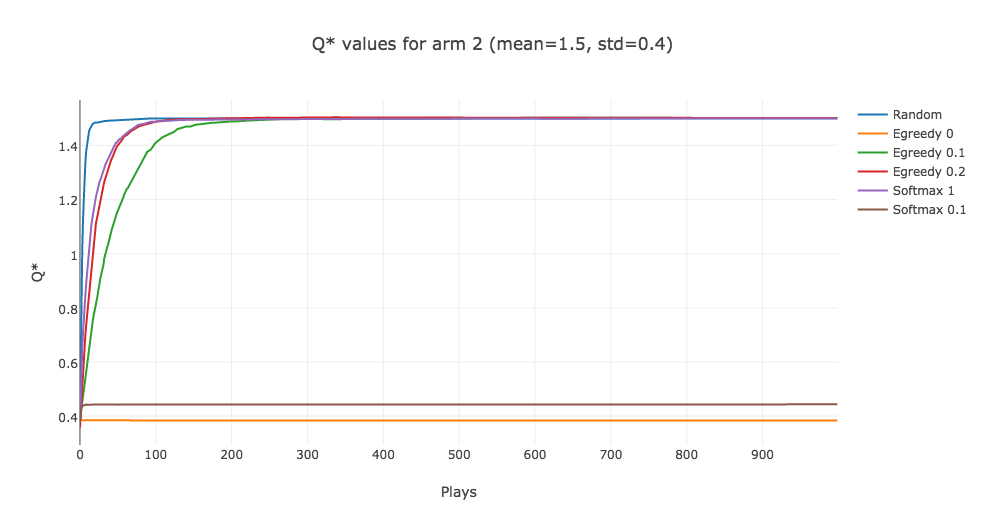
\includegraphics[width=0.7\textwidth]{img/1-1/q3.png}
\end{figure}


\begin{figure}[H]
   \centering
   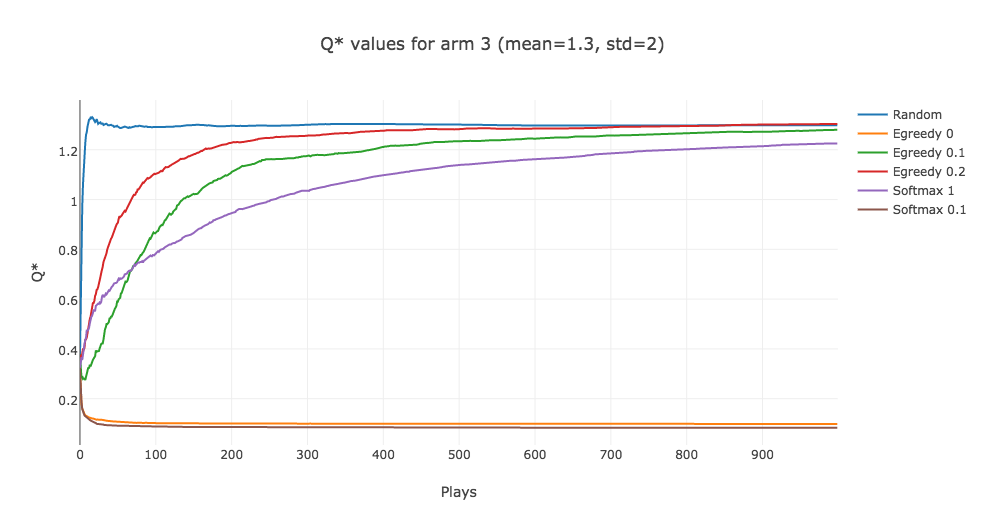
\includegraphics[width=0.7\textwidth]{img/1-1/q4.png}
\end{figure}


\subsubsection{Histogram}

\begin{figure}[H]
   \centering
   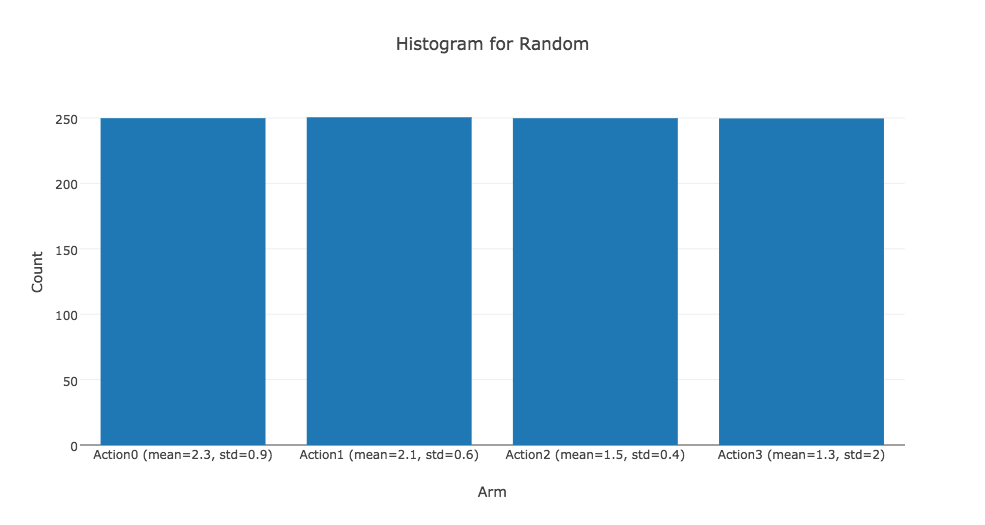
\includegraphics[width=0.7\textwidth]{img/1-1/h1.png}
\end{figure}

\begin{figure}[H]
   \centering
   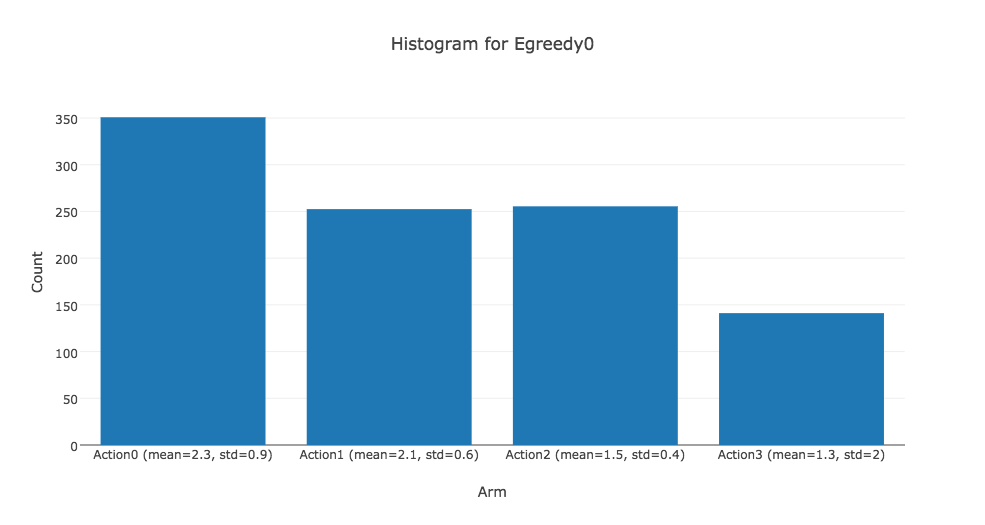
\includegraphics[width=0.7\textwidth]{img/1-1/h2.png}
\end{figure}

\begin{figure}[H]
   \centering
   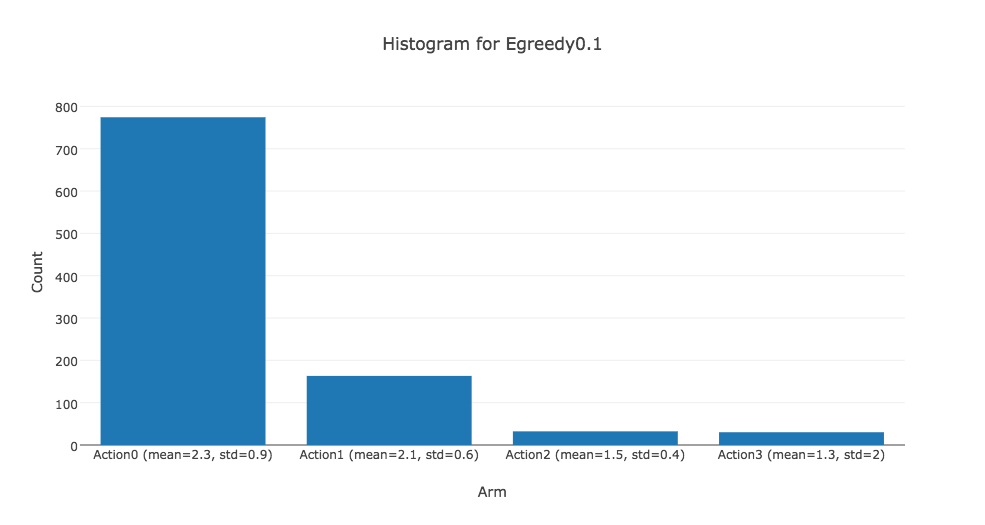
\includegraphics[width=0.7\textwidth]{img/1-1/h3.png}
\end{figure}

\begin{figure}[H]
   \centering
   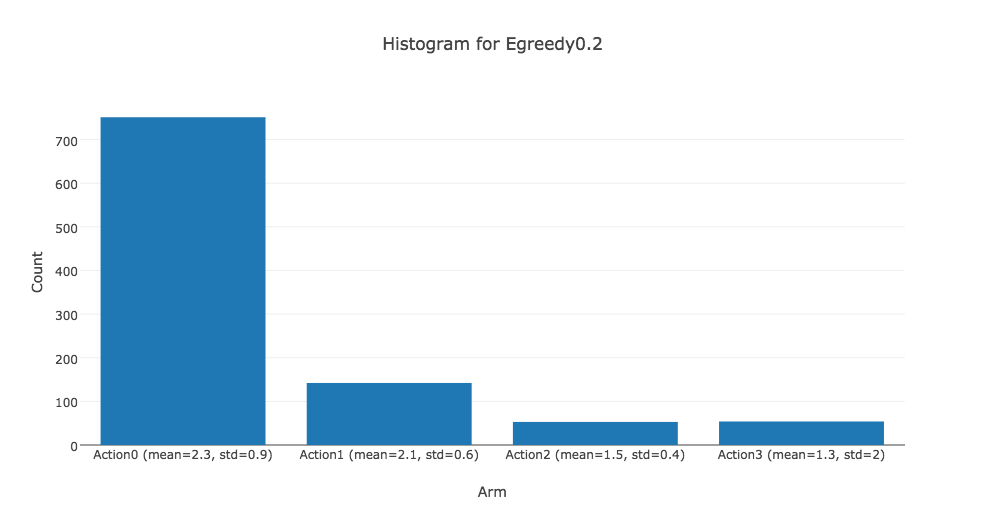
\includegraphics[width=0.7\textwidth]{img/1-1/h4.png}
\end{figure}

\begin{figure}[H]
   \centering
   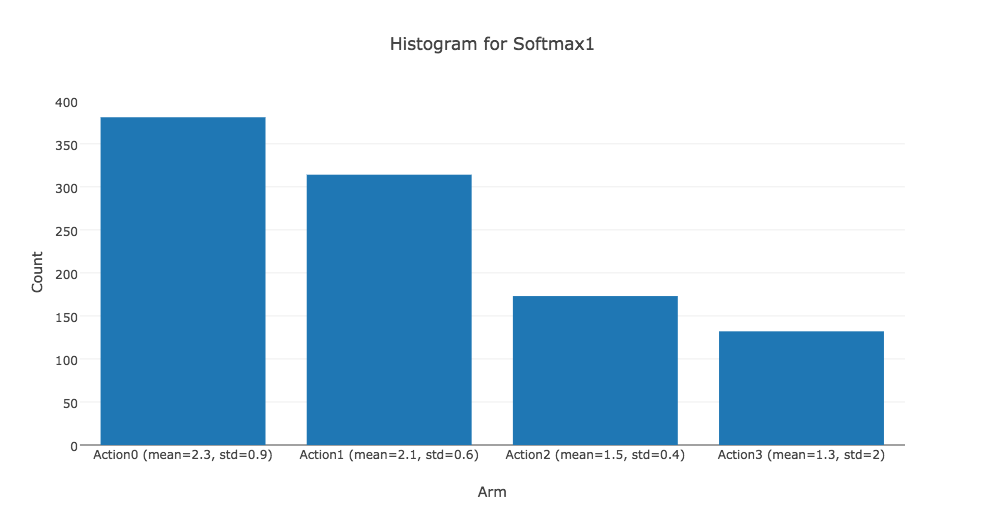
\includegraphics[width=0.7\textwidth]{img/1-1/h5.png}
\end{figure}

\begin{figure}[H]
   \centering
   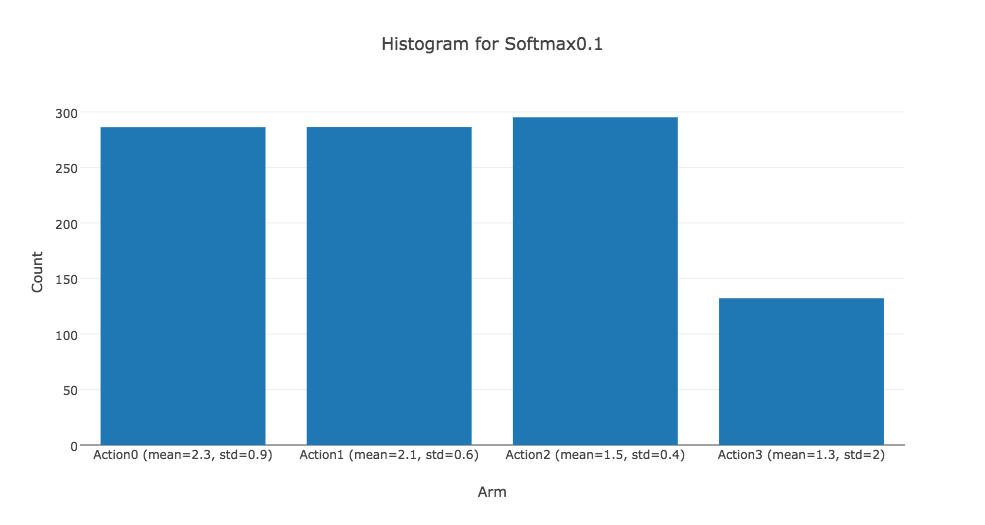
\includegraphics[width=0.7\textwidth]{img/1-1/h6.png}
\end{figure}


\subsubsection{Results}

The average reward graph tends to show that the $\epsilon-greedy$ algorithm tends to choose wisely between the arms and yield the best result (except the one with $\epsilon = 0$ ). 
It is then followed by softmax with 
$\tau = 1$ 
with a poorer performance.
$ \epsilon -greedy 0$ 
and 
$softmax \tau 1$ 
seems not to perform significantly better than the random selector.

The 4 graph representing the evolution of $Q(a)$ for each arm tend to show that all algorithms except $ \epsilon-greedy 0$ and $ softmax \tau 1$ approach the true value $Q*$ in theirs estimations.

The histogram explained the result above. Without surprise, algorithms that tend to yield the best result choose better arm more often.

\subsection{Exercice 2}

\subsubsection{Average reward for each algorithm}

\begin{figure}[H]
   \centering
   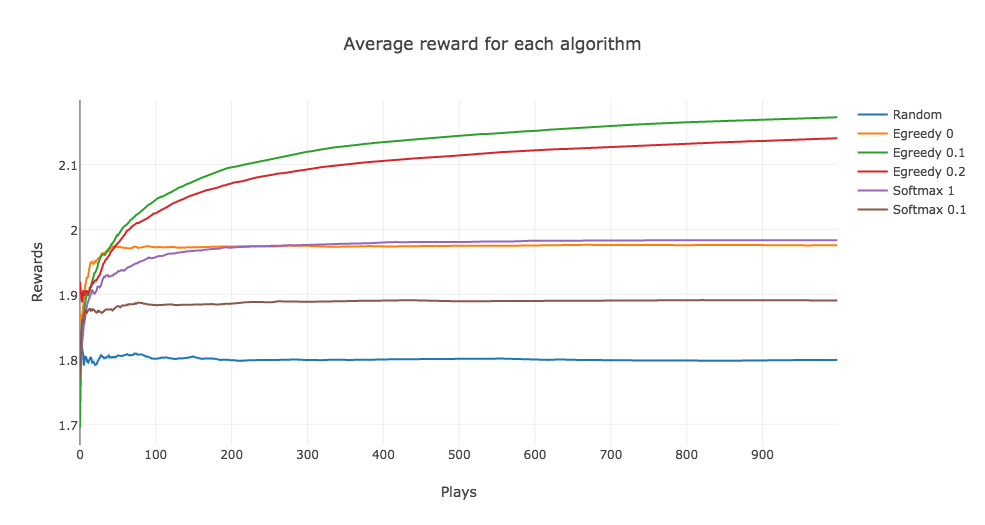
\includegraphics[width=0.8\textwidth]{img/1-2/reward.png}
\end{figure}

\subsubsection{Plot per arm}

\begin{figure}[H]
   \centering
   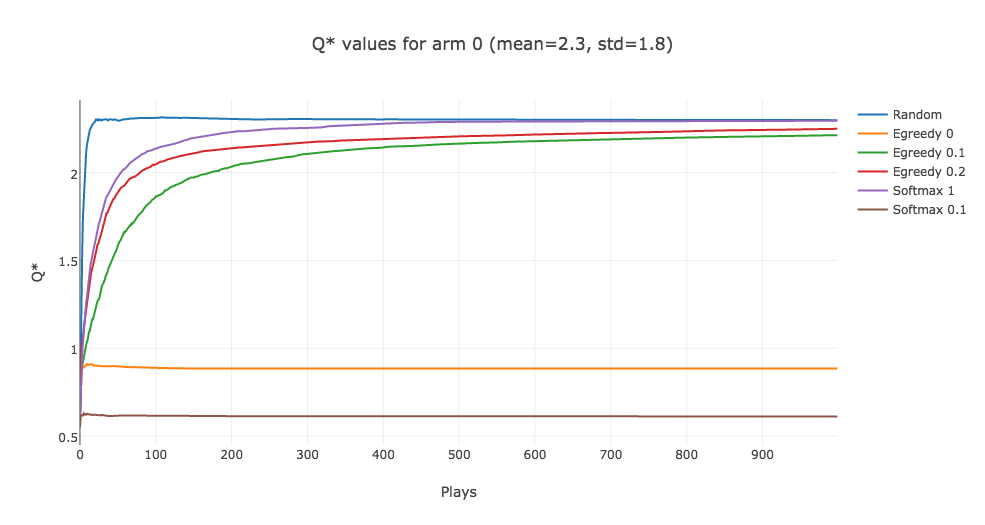
\includegraphics[width=0.7\textwidth]{img/1-2/q1.png}
\end{figure}

\begin{figure}[H]
   \centering
   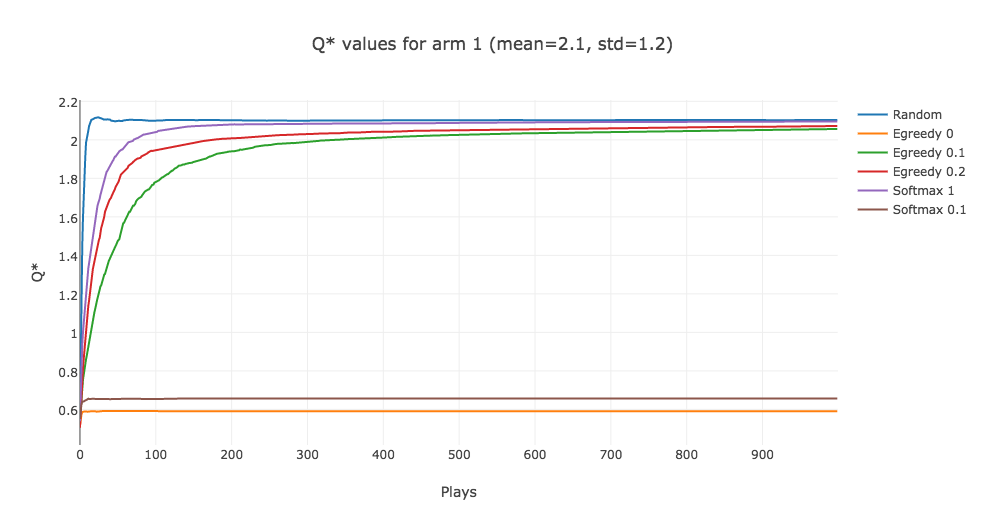
\includegraphics[width=0.7\textwidth]{img/1-2/q2.png}
\end{figure}

\begin{figure}[H]
   \centering
   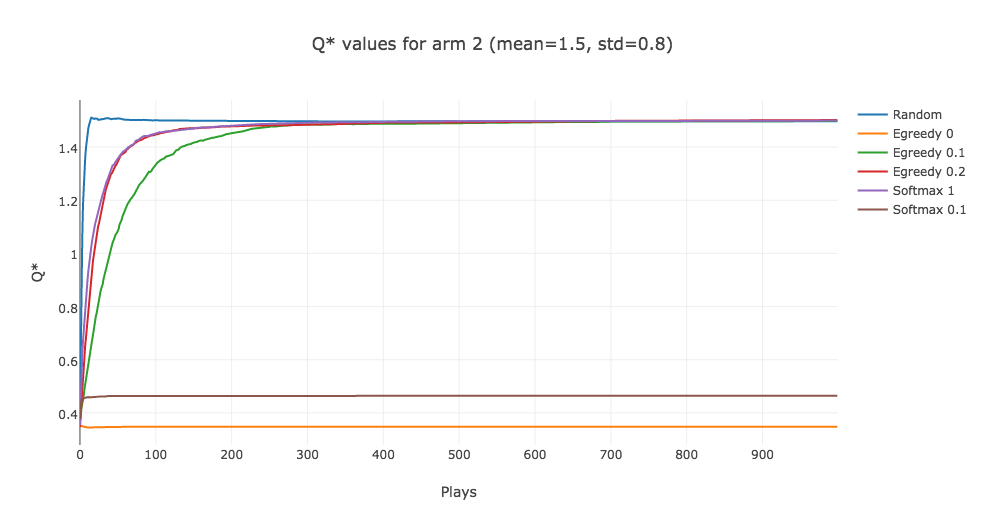
\includegraphics[width=0.7\textwidth]{img/1-2/q3.png}
\end{figure}


\begin{figure}[H]
   \centering
   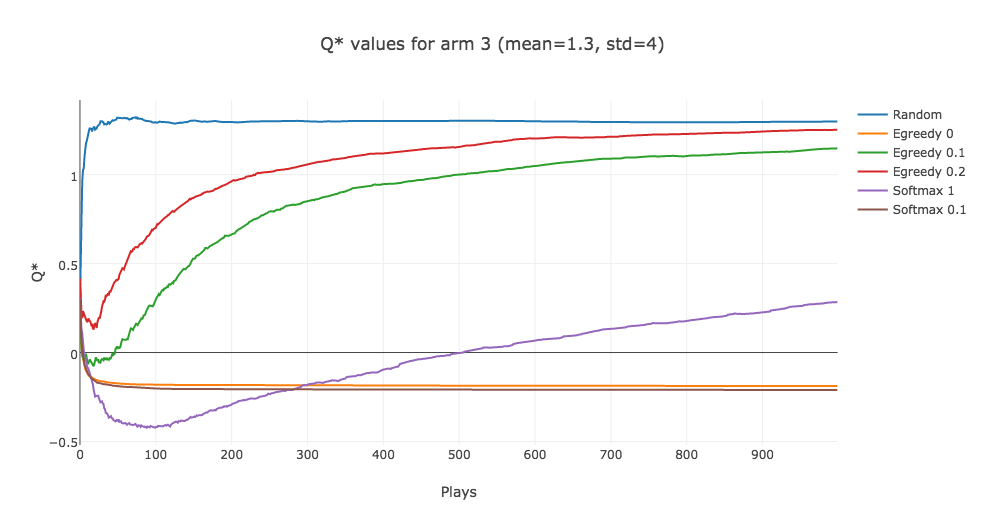
\includegraphics[width=0.7\textwidth]{img/1-2/q4.png}
\end{figure}


\subsubsection{Histogram}

\begin{figure}[H]
   \centering
   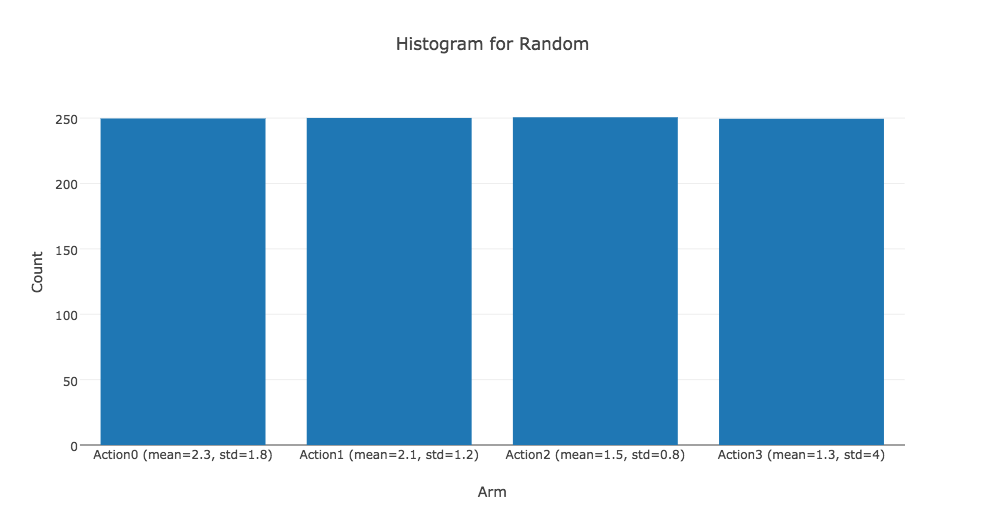
\includegraphics[width=0.7\textwidth]{img/1-2/h1.png}
\end{figure}

\begin{figure}[H]
   \centering
   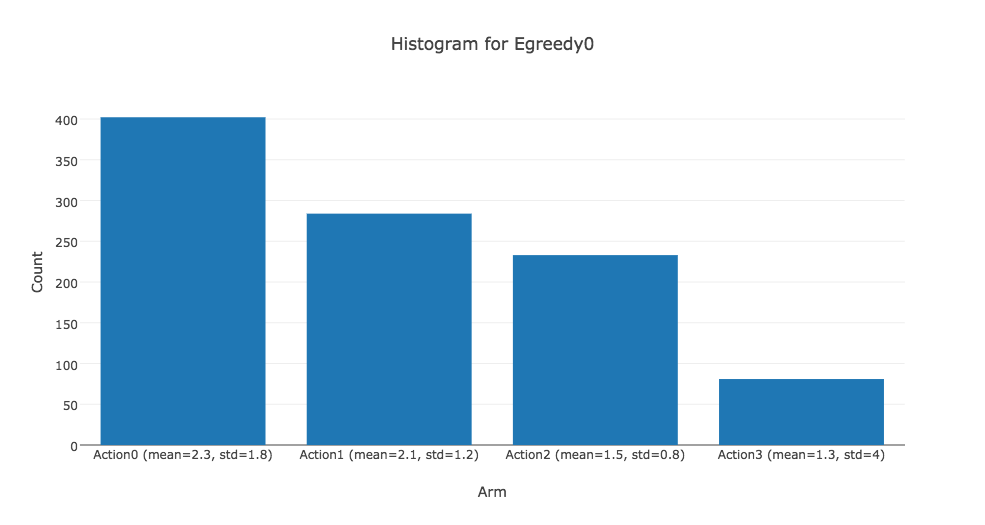
\includegraphics[width=0.7\textwidth]{img/1-2/h2.png}
\end{figure}

\begin{figure}[H]
   \centering
   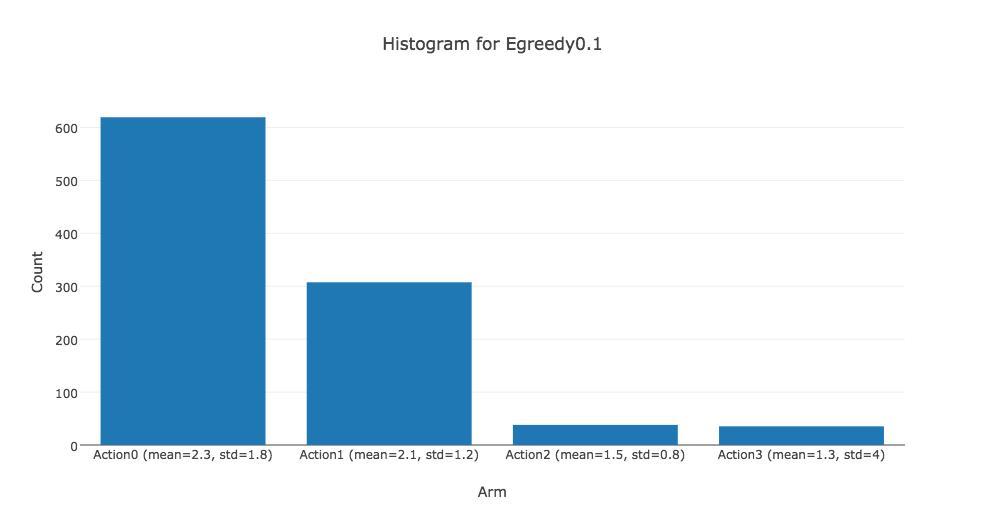
\includegraphics[width=0.7\textwidth]{img/1-2/h3.png}
\end{figure}

\begin{figure}[H]
   \centering
   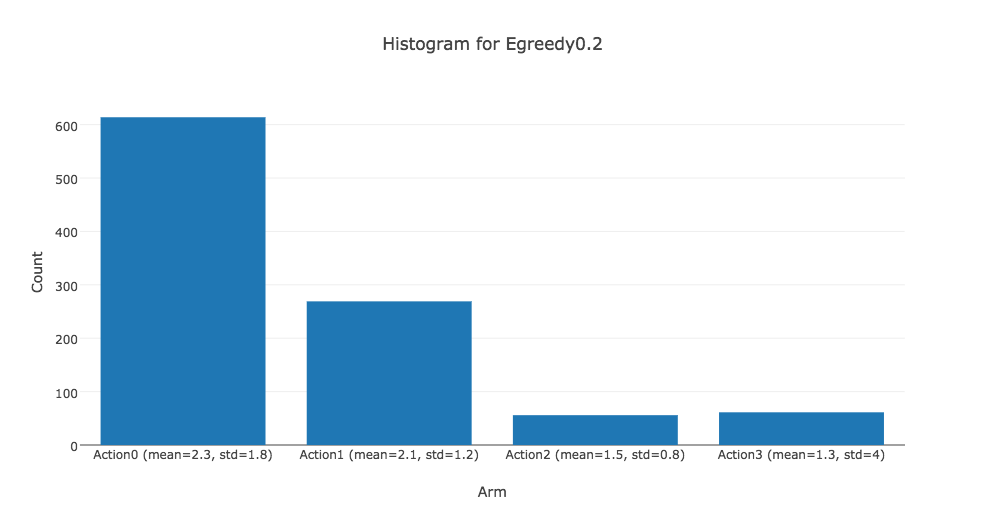
\includegraphics[width=0.7\textwidth]{img/1-2/h4.png}
\end{figure}

\begin{figure}[H]
   \centering
   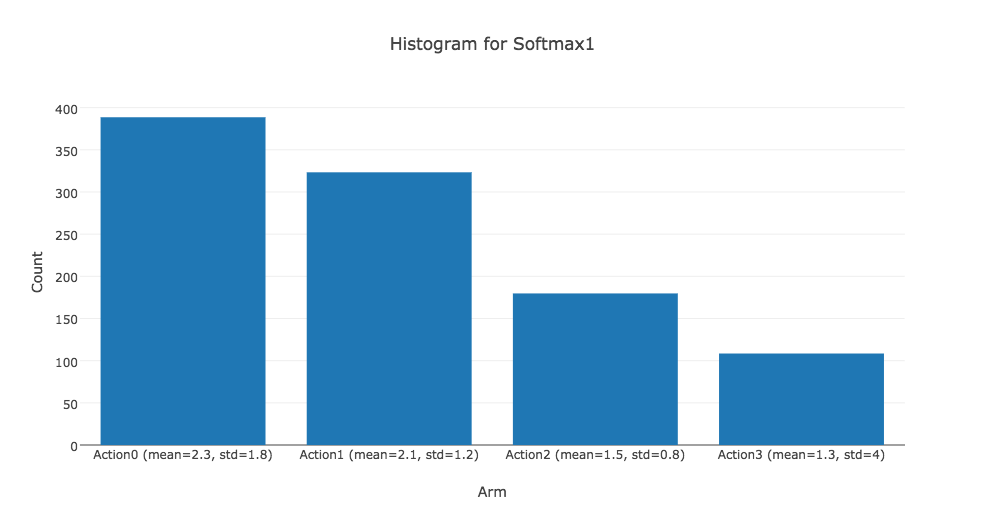
\includegraphics[width=0.7\textwidth]{img/1-2/h5.png}
\end{figure}

\begin{figure}[H]
   \centering
   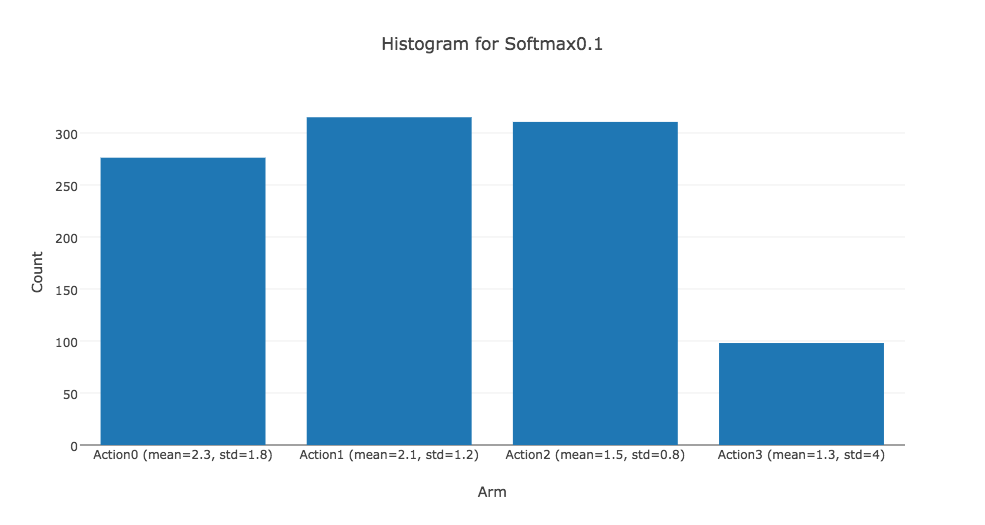
\includegraphics[width=0.7\textwidth]{img/1-2/h6.png}
\end{figure}


\subsubsection{Results}

The higher variance has mainly the effect of making it harder for the algorithms to determine $Q*$ and in other word to understand which one of the arm is better. Indeed, the number of plays needed to converge is increased and thus making the average reward on all the play from the beginning slightly smaller. However, the algorithms that yielded result on small variance still yield a similar result on high variance.

\subsection{Exercice 3}


\subsubsection{Average reward for each algorithm}

\begin{figure}[H]
   \centering
   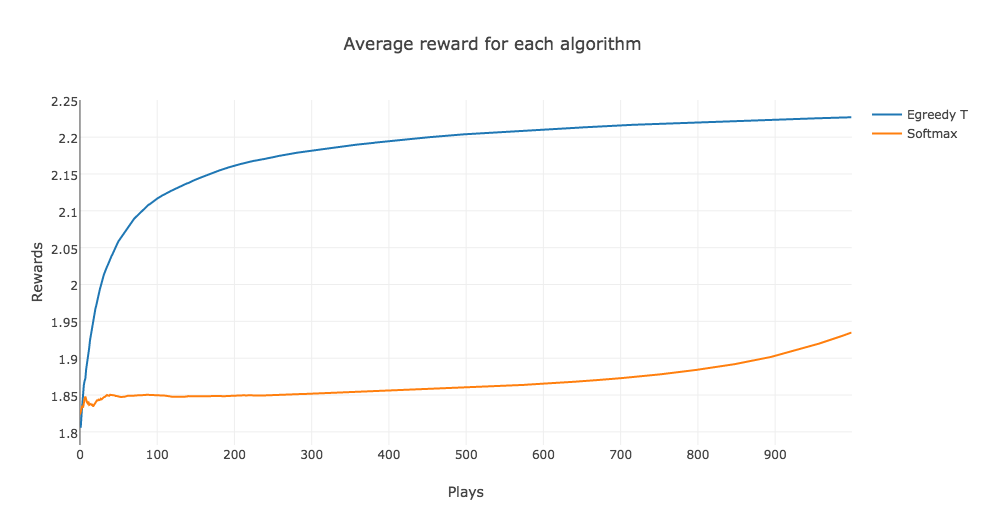
\includegraphics[width=0.8\textwidth]{img/1-3/reward.png}
\end{figure}

\subsubsection{Plot per arm}

\begin{figure}[H]
   \centering
   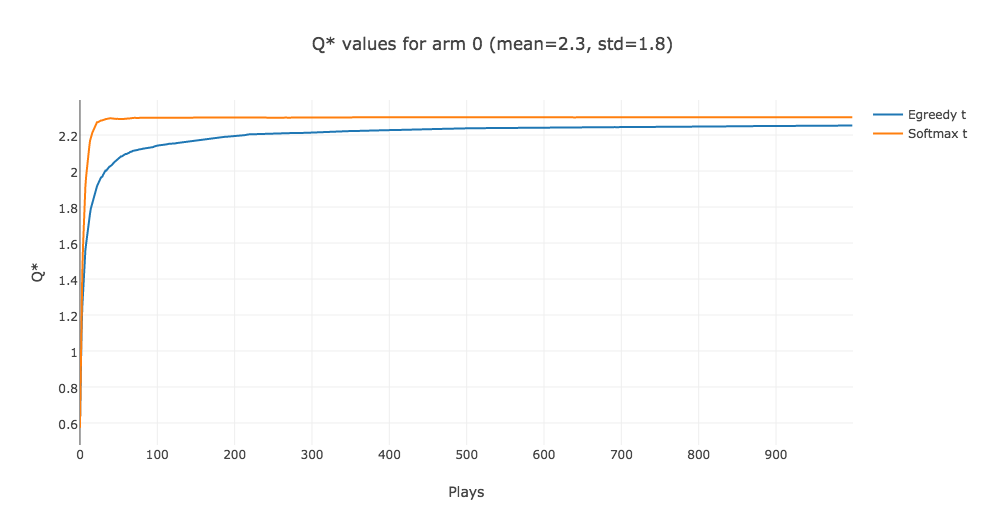
\includegraphics[width=0.7\textwidth]{img/1-3/q1.png}
\end{figure}

\begin{figure}[H]
   \centering
   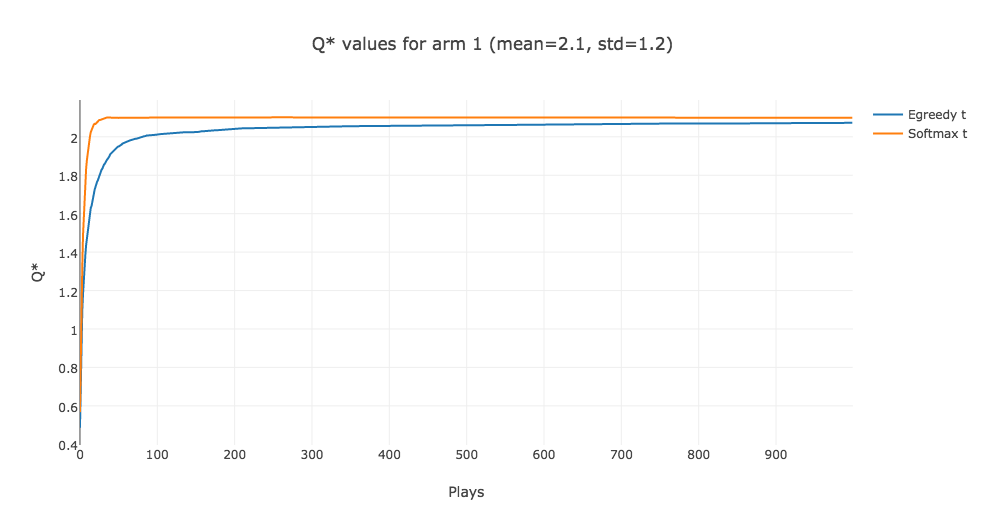
\includegraphics[width=0.7\textwidth]{img/1-3/q2.png}
\end{figure}

\begin{figure}[H]
   \centering
   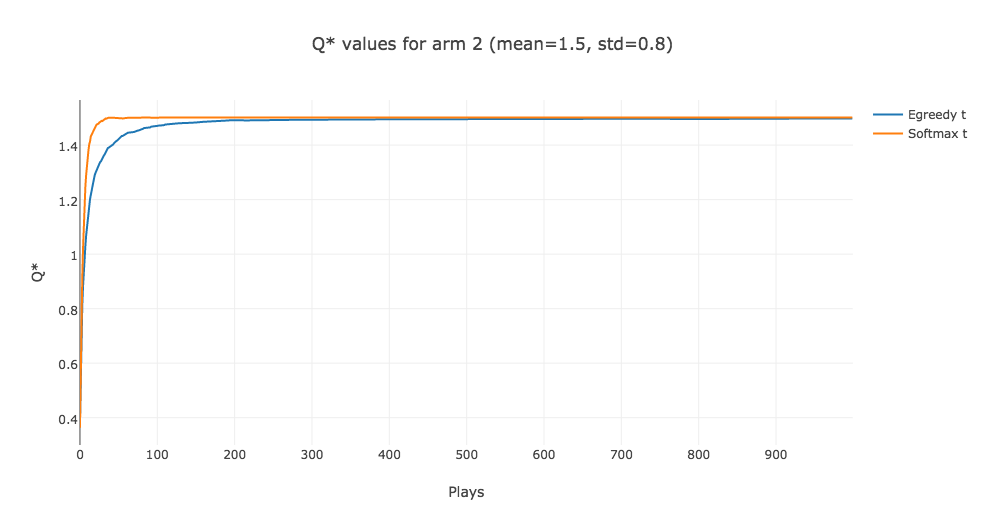
\includegraphics[width=0.7\textwidth]{img/1-3/q3.png}
\end{figure}


\begin{figure}[H]
   \centering
   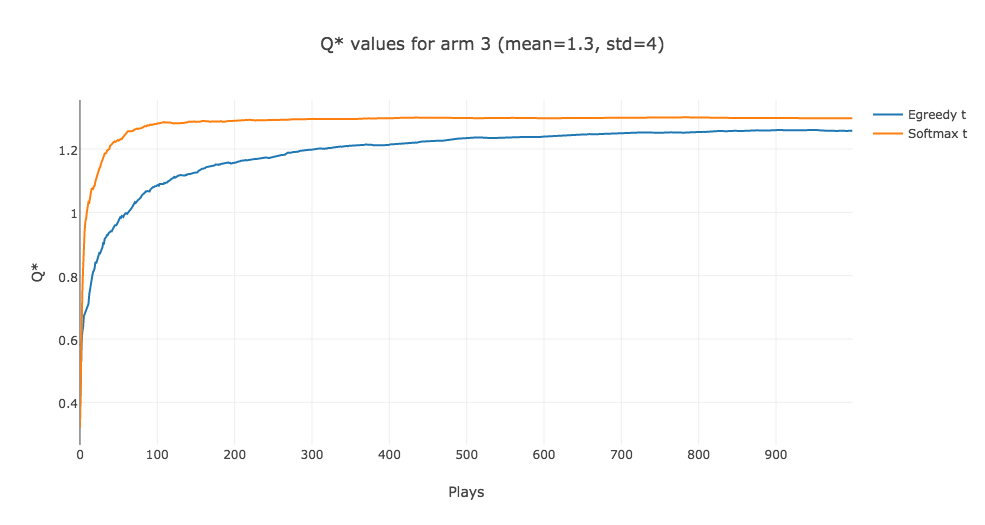
\includegraphics[width=0.7\textwidth]{img/1-3/q4.png}
\end{figure}

\subsubsection{Histogram}

\begin{figure}[H]
   \centering
   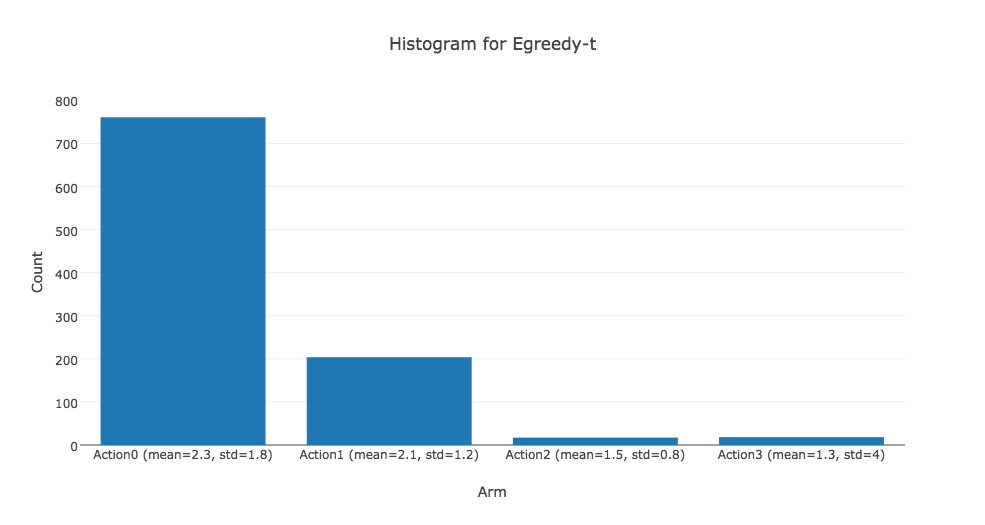
\includegraphics[width=0.7\textwidth]{img/1-3/h1.png}
\end{figure}

\begin{figure}[H]
   \centering
   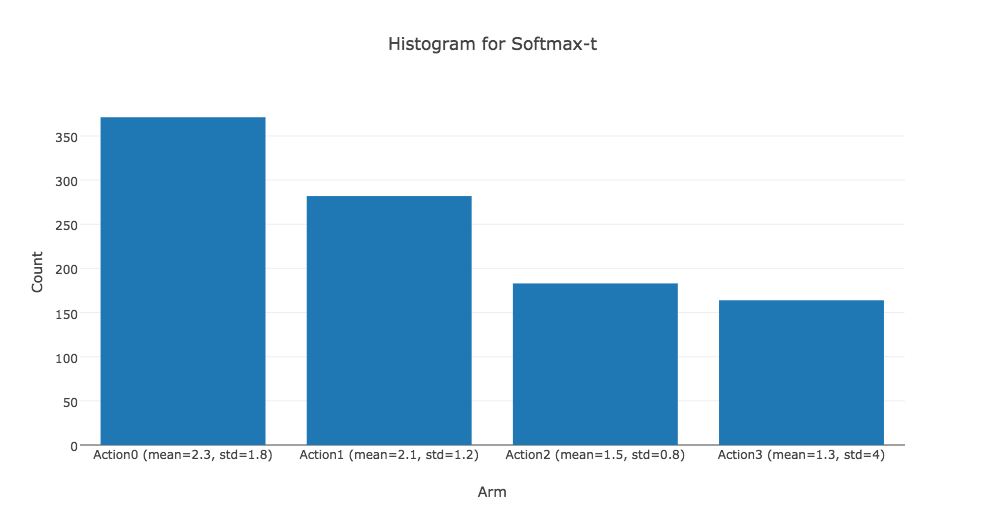
\includegraphics[width=0.7\textwidth]{img/1-3/h2.png}
\end{figure}

\subsubsection{Results}

This techniques here is quite interesting because it allows to make a lot of exploration at the beginning and reduce exploring when the number of play increases. If the parameters are chosen wisely, it would allows to "lock" the algorithms in a optimal state when reached and only exploit this optimal state.

Here we can see that it worked quite well with the $Egreedy T$ but not so well with the $softmax T$ .

\section{Stochastic Reward Game}


\subsection{Plot}

\subsubsection{Std=0.2}

\begin{figure}[H]
   \centering
   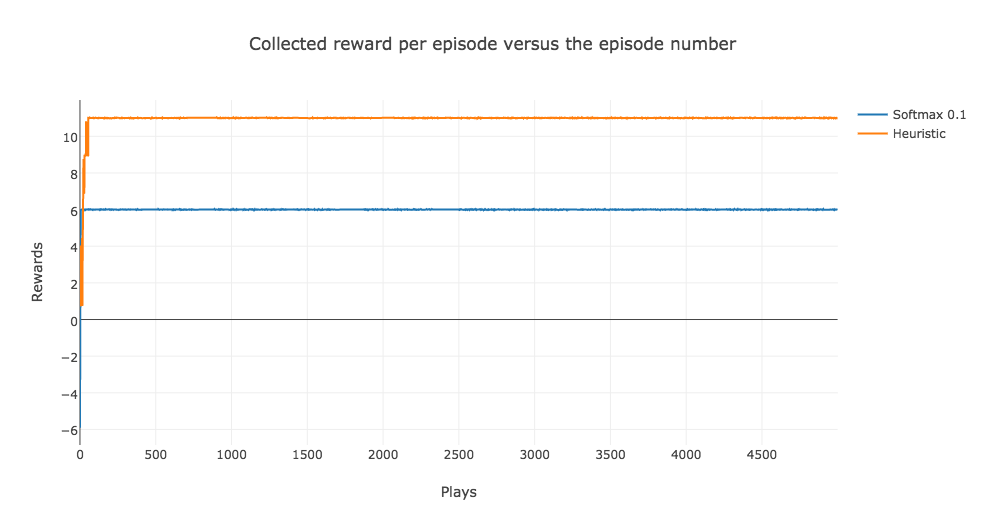
\includegraphics[width=0.7\textwidth]{img/2/1.png}
\end{figure}

\subsubsection{Std=0.1 and std0=4}

\begin{figure}[H]
   \centering
   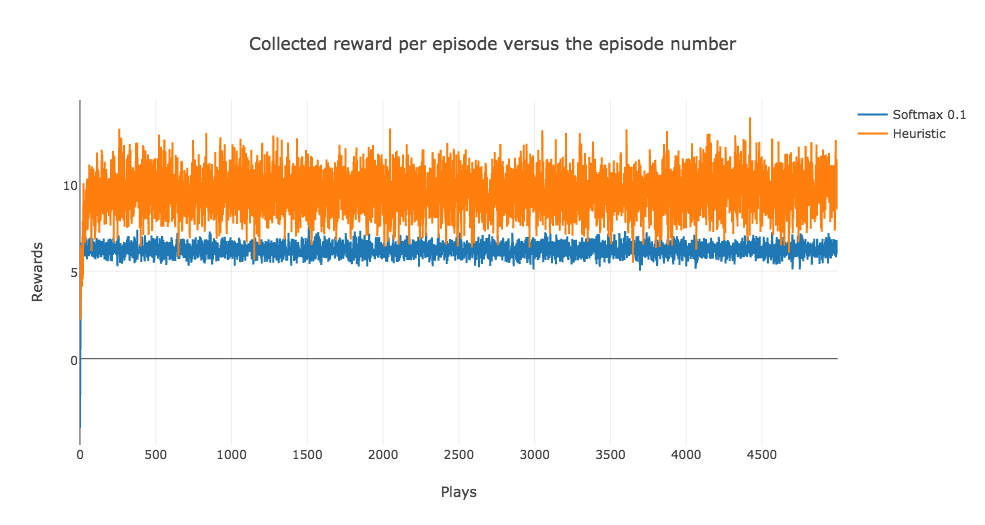
\includegraphics[width=0.7\textwidth]{img/2/2.png}
\end{figure}

\subsubsection{Std=0.1 and std1=4}

\begin{figure}[H]
   \centering
   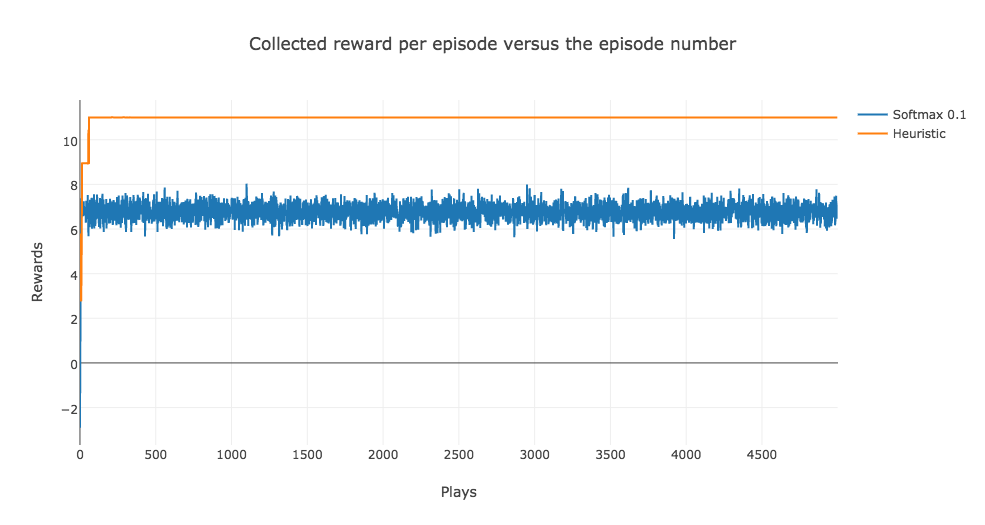
\includegraphics[width=0.7\textwidth]{img/2/3.png}
\end{figure}

\subsubsection{Discussion}

The temperature for the first type with simple Boltzmann action selection has been arbitrarily set.

According to \cite{bestref} and what we can see from the early stage on the graph, the two players begin by playing the non nash equilibrium strategy $<3,3>$.Then when the exploration continues, the two player will find the more attractive but still not equilibrium $<3,2>$. Finally, when exploration continus, the two player will find the non-optimal equilibrum strategy $<2,2>$ and remains there forever. There a not willing to go to a strategy where the loss would be huge $(-30)$ and thus will never reach the optimal equilirbrium $<1,1>$

The heuristic is what \cite{bestref} called \textit{Combined}. It's a combined result of the boltzmann above with a proportion $\rho$ of the MaxQ factor to bias exploration toward actions that have potential to yield higher reward ($11$ in our case).

By looking at the plot, the heuristic seems to be the best action to choose if one want to reach the optimal equilibrium even if the variance is high for this equilibrium.


\subsection{Discussion}

\subsubsection{JAL vs IL}


Independent learners apply Q-learning in the same way as in the bandit problem ignoring the action played by the other player. In the other hand, joint action learners apply Q-learning with the value of their own actions and also with knowledge of other agents actions.

According to \cite{bestref}, if we make the agents independent learner, it will mainly have to effect :
\begin{itemize}
	\item IL would converge slower to a probability of choosing the best action (optimal equilibrium).
	\item IL would have a smaller probability to converge to the optimal equilibrium if the penalty are getting more negative.
\end{itemize}

\subsubsection{Always select the action that yield the highest reward}

This question could be interpreted in more than one way since the part \textit{"the action that according to them will yield the highest reward"} is not clearly defined. The way is what understand is that one player stop or don't do exploration and fixed his action. In that case the other player will choose the best response, his best action possible for the action selected by the other player. There is in this case, no garantee of convergence to an equilibrium (e.g. the player 1 choose to play only $3$, then player 2 will choose to also play $3$ and they will be sticked in $<3,3>$ which is not a equilibrium.


\printbibliography

\end{document}







































              